\chapter{Metamodel dla języka CAL}

Aby otrzymać graficzny edytor modeli wykorzystując \emph{Sirius Web} należy
najpierw zaprojektować metamodel \gls{EMF} opisujący strukturę modeli oraz ich
reprezentację graficzną, która później będzie możliwa do modyfikacji prze
użytkowników. W tym rozdziale
zostanie omówiony język \acrfull{CAL} służący do opisu obliczeń w systemie
\emph{BalticLSC}, a~następnie omówiony zostanie przygotowany metamodel
\gls{EMF}.

\section{Język opisu obliczeń w BalticLSC}

Obliczenia rozproszone wykonywane przez system \emph{BalticLSC} są zapisywane w
formie \emph{aplikacji obliczeniowej} (\emph{computation application})
korzystajac ze składni języka \acrfull{CAL} przygotowanego dla tego właśnie
systemu.

Podstawowym obiektem, który wysyła (wyjście)
lub odbiera (wejście) dane, jest \emph{port}. Jest on reprezentowany za pomocą
ikony kwadratu ze strzałką skierowaną w prawą stronę. Aplikacja obliczeniowa
składa
się z modułów obliczeniowych posiadających swoje porty, portów samej aplikacji
obliczeniowej, oraz połączeń między tymi portami. Grot połączenia wskazuje
kierunek przepływu danych.
Porty aplikacji obliczeniowej są zaznaczone na
diagramie ikoną portu (strzałką skierowaną w prawo) z pogrubioną
jedną z krawędzi ikony --- lewą dla wejścia, prawą dla wyjścia.

Porty modułów oraz aplikacji obliczeniowych mają różne ikony, które
są ustalane na~podstawie ich właściwości. Są dwa kryteria wpływające na ikonę:

\begin{itemize}
	\item różne krotności danych, które obsługuje port: dla pojedynczego pliku będzie to~pojedyncza strzałka, a dla katalogu --- wiele strzałek,
	\item różną liczbę pakietów przyjmowanych lub wysyłanych danych (czy oczekuje pojedynczego zestawu danych wejściowych, czy moduł obsłuży kolejne zestawy danych wysyłane po chwili bez ponownego uruchomienia).
\end{itemize}

Moduł obliczeniowy rozpoczyna obliczenia dopiero gdy na każdym jego wejściu
znajdują się dane.

Przykładowe aplikacje obliczeniowe zostały przedstawaione na
rysunkach~\ref{rys:sekwencyjna-aplikacja-obliczeniowa}
i~\ref{rys:mozliwa-do-zrownoleglenia-aplikacja-obliczeniowa}.
Pierwsza z nich (rysunek~\ref{rys:sekwencyjna-aplikacja-obliczeniowa}) jest
aplikacją, w której obliczenia mogą zostać wykonane
wyłącznie sekwencyjnie, ponieważ dane przepływają sekwencyjnie od wejścia
kolejno przez moduły nazwane \texttt{VideoToFrames}, \texttt{Face Detector},
\texttt{Blur Module}, \texttt{Blur module}, aż w końcu trafiają do wyjścia.
Inna jest struktura aplikacji na
rysunku~\ref{rys:mozliwa-do-zrownoleglenia-aplikacja-obliczeniowa}. Tam
przepływ danych rozdziela się~po~module obliczeniowym \texttt{Pdf page
	splitter} i obliczenie modułów \texttt{OCT Tesseract Tess 0.1} oraz
\texttt{OCR Tesseract LSTM 0.1} może zostać wykonane równolegle, być może
przez różne węzły obliczeniowe. Ich wyniki trafią później do modułu \texttt{Pdf
	data joiner 0.1} i przejdą dalej przez pozostałe moduły w sposób
sekwencyjny.

\begin{figure}[!ht]
	\centering

	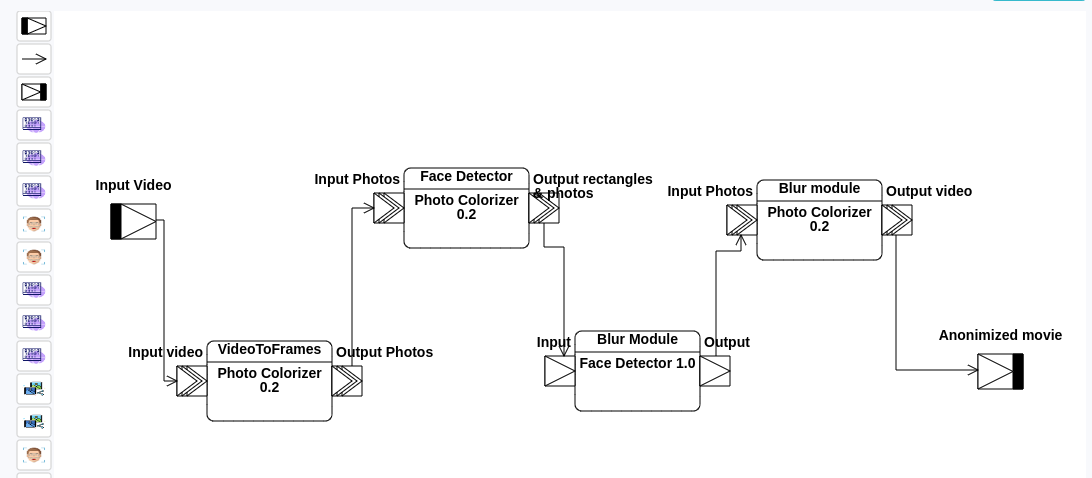
\includegraphics[width=0.95\linewidth]{./images/balticlsc-example-diagram.png}
	\caption{Aplikacja obliczeniowa w BalticLSC z obliczeniami
		sekwencyjnymi.}\label{rys:sekwencyjna-aplikacja-obliczeniowa}
\end{figure}

% \begin{noindent}
\begin{figure}[!ht]
	\centering

	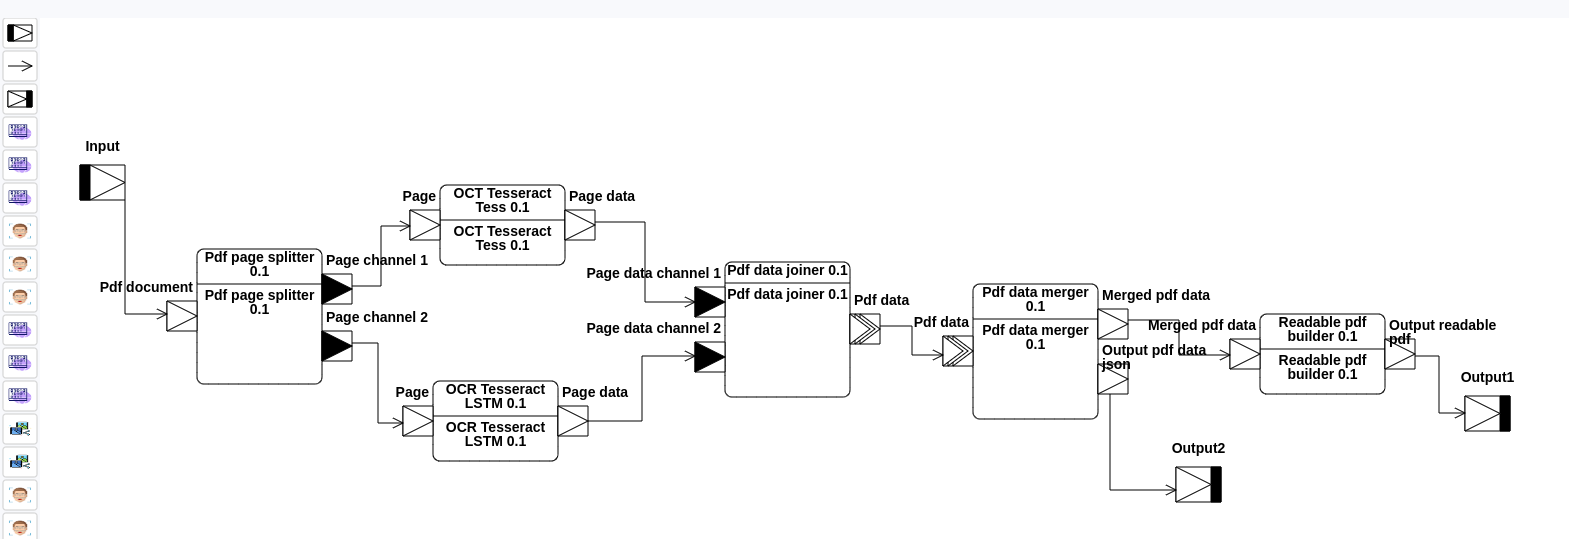
\includegraphics[width=0.99\linewidth]{./images/balticlsc-concurrent-application-example.png}
	\caption{Aplikacja obliczeniowa w BalticLSC z możliwością
		zrównoleglenia obliczeń.}\label{rys:mozliwa-do-zrownoleglenia-aplikacja-obliczeniowa}
\end{figure}
% \end{noindent}

\section{Stworzony metamodel EMF dla języka CAL}

Omówienie przygotowanego modelu. Zrzut ekranu przedstawiający model. Omówienie
elementów oraz jakie one mają przełożenie na wykonanie obliczeń przez
BalticLSC\@.

\subsection{Warunkowa zmiana stylu elementów}

Omówienie reguł warunkowej zmiany stylu elementów diagramu:

\begin{enumerate}
	\item \texttt{DataPin} zmieniają ikonę na podstawie swoich \textit{data
		      multiplicity} oraz \textit{token multiplicity}.
	\item \texttt{ComputedDataPin} zmieniają kolor na podstawie swojego
	      \textit{data binding}.
\end{enumerate}

\subsection{Narzędzia edytora diagramów}

Omówienie dodanych \textit{Tools} z Sirius:

\begin{itemize}
	\item usunięcie \texttt{UnitCall} lub \texttt{ApplicationDataPin} usuwa również powiązane \texttt{DataFlow}
	\item usunięcie \texttt{ComputedDataPin} z poziomu edytora diagramów nie jest możliwe
	\item ograniczenia na tworzenie \texttt{DataFlow} tak, aby były semantycznie poprawne
	\item automatyczne usuwanie i tworzenie \texttt{ComputedDataPin} po zmianie \texttt{ComputationUnitRelease} dla danego \texttt{UnitCall}
	\item okno dialogowe ułatwiające tworzenie \texttt{UnitCall} dla istniejącego \texttt{ComputationUnitRelease}
	\item \ldots
\end{itemize}

\subsection{Reguły walidacyjne powiązane z
	metamodelem}\label{sec:regulky-walidacyjne-metamodel}

Omówienie \textit{semantic validation rule} z pliku \texttt{*.odesign}, które
działają w Sirius Desktop.

\subsection{Testy metamodelu}

Omówienie dodanych testów jednostkowych modelu (głównie dotyczy automatycznego
zarządzania \texttt{ComputedDataPin} w zależnosci od
\texttt{ComputationUnitRelease} dla konkretnego \texttt{UnitCall}).
